\section{Challenges Faced in Azure CI-CD Implementation [Rahat Rafiq]}\label{sec:challenges_faced_in_azure_ci_cd}

\subsection{Test DB Connection}

Since the application properties of the spring boot application were reconfigured to connect to a PostgreSQL database instead of an embedded H2 database, all the test cases in the CI pipeline was failing to pass with a bean creation exception error. The application properties file was edited to accommodate a PostgreSQL database because software development best practices suggest developers to always build and test the application in the local machine before pushing it to a version control repository. Even though the CI pipeline will essentially build the application again, it is a good idea to pre-check it to avoid failed executions. Because otherwise, the source repository will need to be rolled back to a previous commit or a new branch created from a previous error-free commit. Which can lead to some serious complications in a large organization project. The primary idea was to connect to the PostgreSQL service container that was already running on the CI pipeline hosted machine. However, in the application properties data source URL, the connection string is defined with localhost. Which does not work in this scenario because in the docker environment a container is assigned an IP address for every Docker network it connects to. The IP address is assigned from the pool assigned to the network, so the Docker daemon effectively acts as a DHCP server for each container. In other words, every time the CI pipeline is executed a new PostgreSQL service container will spin up with a different IP address.

The solution to the problem is to fetch the IP address of the PostgreSQL service container for each CI build. The IP address can be fetched using the docker inspect command with a customized query string to return just the IP address of the container and store that in a variable. Then in the data source URL localhost is replaced with this IP address variable. Now the application will be able to successfully connect to the PostgreSQL service container and run all the test cases. ~\ref{fig:fetch_pgsql_IP} 

\begin{figure}
    \centering
    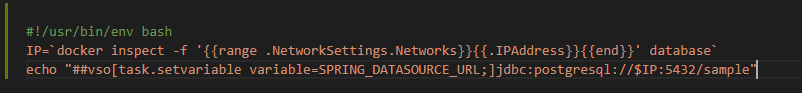
\includegraphics[width=14cm]{images/Rahat/C1.PNG}
    \caption{Docker Fetch Postgresql IP}
    \label{fig:fetch_pgsql_IP}
\end{figure}


\subsection{Service Connection Automation}

CI-CD pipeline implementation in azure is a culmination of two services. Azure cloud portal and Azure DevOps. The pipeline is executed in the DevOps service but all the resources including container registries and Kubernetes cluster are deployed in the azure cloud portal. Thus it is essential to configure several service connections from azure DevOps to the azure cloud portal. Each service connection will create a service principal account, which will be used by the CI-CD pipeline to log into specific azure cloud portal resources and deploy containers and clusters. The process of creating service connections from the portal is fairly straightforward. However, since this task is needed to be executed multiple times in the pipeline, it would be a good idea to achieve some automation here. ARM template can be used to deploy the azure service but unfortunately it can not used be to create a service connection in Azure DevOps. 

The only solution to achieve automation in this aspect is to send HTTP requests to azure DevOps REST API endpoints using a PowerShell script from the pipelines. The script will call the API two times to achieve this goal. The first call is to get the project ID because an API call body is needed. The second time is to create a service connection at the project level. ~\ref{fig:service_principal_automation}

\begin{figure}
    \centering
    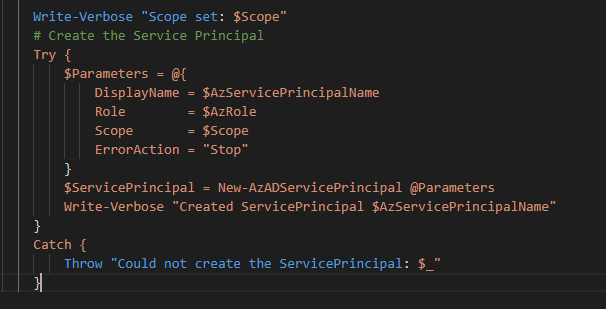
\includegraphics[width=12cm]{images/Rahat/C2.PNG}
    \caption{Service Principal automation}
    \label{fig:service_principal_automation}
\end{figure}


